% ----------------------------------------------------------
\chapter{Fundamentação Teórica}\label{cap:fundamentacao_teorica}
% ----------------------------------------------------------

% \textbf{Instruções da Coordenação do PFC:}

% Deve-se colocar um parágrafo introdutório no início de \textbf{cada} capítulo, descrevendo os assuntos que serão abordados e a relação com o restante do trabalho. Por exemplo: \emph{A Seção 2.1 apresenta \ldots. Os resultados obtidos são analisados na Seção 2.2.} Pode-se fazer o mesmo no início de seções maiores, explicando para o leitor, em uma ou duas sentenças, o que está por vir no texto e o porquê. Outra boa prática é, ao final de cada capítulo, fazer uma ligação com o capítulo seguinte por meio de parágrafo curto.

% Neste capítulo, deve-se apresentar as principais teorias, conceitos, técnicas, modelos, etc que são essenciais para o entendimento do problema tratado e da solução proposta.

% Figuras, tabelas, quadros e equações devem ser introduzidos e explicados no texto: não se pode simplesmente ``jogá-los'' no texto, sem referência nem explicação. Por exemplo, deve-se escrever algo como: \emph{O circuito projetado é mostrado na Figura~10. O resistor $R_1$ faz o papel de um limitador de corrente, enquanto o capacitor $C_2$ juntamente com o resistor $R_5$ formam um filtro passa-baixa. Este circuito tem a vantagem de \ldots}

% Com relação às equações, não se faz referência a uma equação que ainda não foi apresentada. Por exemplo, não se escreve: \emph{A relação entre a tensão e a corrente de um resistor é dada pela \autoref{eq:leiDeOhm}:}
% \begin{equation}\label{eq:leiDeOhm}
%     V = R I \, \text{.}
% \end{equation}

% \noindent O correto é algo como: \emph{A relação entre a tensão e a corrente de um resistor é dada por (Lei de Ohm)}
% \begin{equation}\label{eq:leiDeOhm2}
%     V = R I \, \text{,}
%    \end{equation}
% \emph{na qual $V$ é a tensão sobre o resistor, $R$ a resistência e $I$ a corrente elétrica. Da \autoref{eq:leiDeOhm2}, obtemos que}
% \begin{equation}\label{eq:leiDeOhm3}
%     I = \dfrac{V}{R} \, \text{.}
% \end{equation}

% \emph{Por outro lado, \ldots}

% É importante observar que as equações fazem parte do texto e, assim, deve-se inserir uma vírgula ou ponto ao seu final. Se o parágrafo segue, pode-se eliminar o recuo na próxima linha com o comando \verb!\noindent!. Além disto, se a frase segue, inicia-se a linha com letra minúscula. Veja os exemplos das Equações~(\ref{eq:leiDeOhm2}) e (\ref{eq:leiDeOhm3}).

% A seguir encontra-se uma equação na linha de texto: $\hat{y}(t+k\mid t)= \sum^\infty_{i=1} g_i \Delta u(t+k-i\mid t)$. E também, mais à frente, um exemplo de referência cruzada da \autoref{fig:Fig_1} e da \autoref{eq:Eq_1}.

% \pagebreak

% \textbf{Instruções do padrão genérico de TCCs da BU:}

% Deve-se inserir texto entre as seções.

% % ----------------------------------------------------------
% \section{Exposição do tema ou matéria}
% % ----------------------------------------------------------

% É a parte principal e mais extensa do trabalho. Deve apresentar a fundamentação teórica, a metodologia, os resultados e a discussão. Divide-se em seções e subseções conforme a NBR 6024 \cite{NBR6024:2012}.

% Quanto à sua estrutura e projeto gráfico, segue as recomendações da \gls{ABNT} para preparação de trabalhos acadêmicos, a NBR 14724, de 2011 \cite{NBR14724:2011}.

% \begin{figure}[htb]
% 	\caption{\label{fig:Fig_1}Elementos do trabalho acadêmico.}
% 	\begin{center}
% 		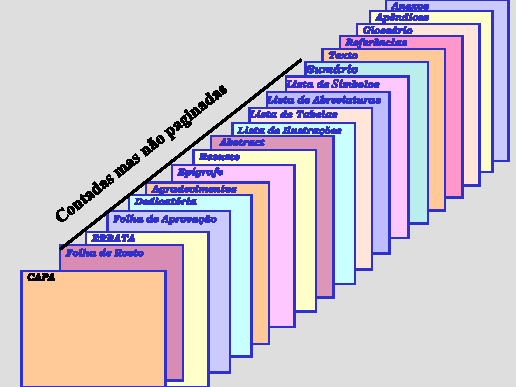
\includegraphics{images/imagem.pdf}
% 	\end{center}
% 	\fonte{Universidade Federal do Paraná (1996).}
% \end{figure}

% % ----------------------------------------------------------
% \subsection{Formatação do texto}
% % ----------------------------------------------------------

% No que diz respeito à estrutura do trabalho, recomenda-se que:
% \begin{alineas}
% 	\item o texto deve ser justificado, digitado em cor preta, podendo utilizar outras cores somente para as ilustrações;
% 	\item utilizar papel branco ou reciclado para impressão;
% 	\item os elementos pré-textuais devem iniciar no anverso da folha, com exceção da ficha catalográfica ou ficha de identificação da obra;
% 	\item os elementos textuais e pós-textuais devem ser digitados no anverso e verso das folhas, quando o trabalho for impresso. As seções primárias devem começar sempre em páginas ímpares, quando o trabalho for impresso. Deixar um espaço entre o título da seção/subseção e o texto e entre o texto e o título da subseção.
% \end{alineas}

% No \autoref{qua:Quadro_1} estão as especificações para a formatação do texto.

% \begin{quadro}[htb]
% 	\centering
% 	\caption{\label{qua:Quadro_1}Formatação do texto.}	
% 	\begin{tabular}{|l|p{11cm}|}
% 		\hline
% 		\textbf{Formato do papel} & A4.\\ \hline
% 		\textbf{Impressão}        & A norma recomenda que caso seja necessário imprimir, deve-se utilizar a frente e o verso da página.\\ \hline
% 		\textbf{Margens}          & Superior: 3, Inferior: 2, Interna: 3 e Externa: 2. Usar margens espelhadas quando o  trabalho for impresso.\\ \hline
% 		\textbf{Paginação}        & As páginas dos elementos pré-textuais devem ser contadas, mas não numeradas. Para trabalhos digitados somente no anverso, a numeração das páginas deve constar no canto superior direito da página, a 2 cm da borda, figurando a partir da primeira folha da  parte textual. Para trabalhos digitados no anverso e no verso, a numeração deve constar no canto superior direito, no anverso, e no canto superior esquerdo no verso.\\ \hline
% 		\textbf{Espaçamento}      & O texto deve ser redigido com espaçamento entre linhas 1,5, excetuando-se as citações de mais de três linhas, notas de rodapé, referências, legendas das ilustrações e das tabelas, natureza (tipo do trabalho, objetivo, nome da instituição a que é submetido e área de concentração), que devem ser digitados em espaço simples, com fonte menor. As referências devem ser separadas entre si por um espaço simples em branco.\\ \hline
% 		\textbf{Paginação}        & A contagem inicia na folha de rosto, mas se insere o número da página na introdução até o final do trabalho.\\ \hline
% 		\textbf{Fontes sugeridas} & Arial ou Times New Roman.\\ \hline
% 		\textbf{Tamanho da fonte} & \textbf{Fonte tamanho 12 para o texto}, incluindo os títulos das seções e subseções. As citações com mais de três linhas, notas de rodapé, paginação, dados internacionais de catalogação, legendas e fontes das ilustrações e das tabelas devem ser de tamanho menor. Adotamos, neste \textit{template} \textbf{fonte tamanho 10}.\\ \hline
% 		\textbf{Nota de rodapé}   & Devem ser digitadas dentro da margem, ficando separadas por um espaço simples por entre as linhas e por filete de 5 cm a partir da margem esquerda. A partir da segunda linha, devem ser alinhadas embaixo da primeira letra da primeira palavra da primeira linha.\\ \hline
% 	\end{tabular}
% 	\fonte{\textcite{NBR14724:2011}.}
% \end{quadro}

% % ----------------------------------------------------------
% \subsubsection{As ilustrações}
% % ----------------------------------------------------------

% Independentemente do tipo de ilustração (quadro, desenho, figura, fotografia, mapa, entre outros), a sua identificação aparece na parte superior, precedida da palavra designativa. 

% \begin{citacao}
% 	Após a ilustração, na parte inferior, indicar a fonte consultada (elemento obrigatório, mesmo que seja produção do próprio autor), legenda, notas e outras informações necessárias à sua compreensão (se houver). A ilustração deve ser citada no texto e inserida o mais próximo possível do texto a que se refere. \cite[p. 11]{NBR14724:2011}.
% \end{citacao}

% % ----------------------------------------------------------
% \subsubsection{Equações e fórmulas}
% % ----------------------------------------------------------

% As equações e fórmulas devem ser destacadas no texto para facilitar a leitura.  Para numerá-las, usar algarismos arábicos entre parênteses e alinhados à direita. Pode-se adotar uma entrelinha maior do que a usada no texto \cite{NBR14724:2011}.

% Exemplos, \autoref{eq:Eq_1} e \autoref{eq:Eq_2}. Observe que o comando \verb|\gls{}| é usado para utilizar para criar um \emph{hyperlink} com a definição do símbolo na lista de símbolos (veja linha 153 de \emph{main.tex}.

% \begin{equation}
% \label{eq:Eq_1}
% \gls{C} = 2 \gls{pi} \gls{r} \sqrt{\gamma} + 10 \, \text{.}
% \end{equation}

% \begin{equation}
% \label{eq:Eq_2}
% \gls{A} = \gls{pi} \gls{r}^2 \, \text{.}
% \end{equation}

% \noindent Aqui não há recuo porque o parágrafo não terminou, apenas foi iniciada uma nova frase após a equação. As equações fazem parte do texto, portanto estão sujeitas à pontuação (ponto final, vírgula etc.).

% % ----------------------------------------------------------
% \subsubsubsection{Exemplo tabela}
% % ----------------------------------------------------------

% De acordo com \textcite{ibge1993}, tabela é uma forma não discursiva de apresentar informações em que os números representam a informação central. Ver \autoref{tab:Tab_1}.

% \begin{table}[htb]
% 	\ABNTEXfontereduzida
% 	\caption{\label{tab:Tab_1}Médias concentrações urbanas 2010-2011.}
% 	\begin{tabular}{@{}p{3.0cm}p{1.5cm}p{2cm}p{2.5cm}p{2.5cm}p{2.5cm}@{}}
% 		\toprule
% 		\textbf{Média concentração urbana} & \multicolumn{2}{l}{\textbf{População}} & \textbf{Produto Interno Bruto – PIB (bilhões R\$)} & \textbf{Número de empresas} & \textbf{Número de unidades locais} \\ \midrule
% 		\textbf{Nome}                      & \textbf{Total}   & \textbf{No Brasil}  &                                                   &                             & \\
% 		Ji-Paraná (RO)                     & 116 610          & 116 610             & 1,686                                             & 2 734                       & 3 082 \\
% 		Parintins (AM)                     & 102 033          & 102 033             & 0,675                                             & 634                         & 683 \\
% 		Boa Vista (RR)                     & 298 215          & 298 215             & 4,823                                             & 4 852                       & 5 187 \\
% 		Bragança (PA)                      & 113 227          & 113 227             & 0,452                                             & 654                         & 686 \\ \bottomrule
% 	\end{tabular}
% 	\fonte{\textcite{ibge2016}.}
% \end{table}

\section{APIs e APIs Restful}

APIs (\textit{Application Programming Interfaces}) são interfaces que permitem a comunicação entre diferentes sistemas, softwares ou componentes. Elas funcionam como pontes que facilitam o intercâmbio de dados e funcionalidades, promovendo integração e interoperabilidade. A ideia de API remonta aos primórdios da computação, quando surgiram as primeiras necessidades de criar padrões para que sistemas independentes pudessem se comunicar. Inicialmente, as APIs eram utilizadas em bibliotecas locais para abstrair funcionalidades complexas de hardware e software. Com o avanço da internet, especialmente nas décadas de 1990 e 2000, as APIs evoluíram para um modelo remoto, permitindo que sistemas distribuídos interagissem de maneira mais eficiente.

Nesse contexto, surgiu o conceito de APIs REST, um estilo arquitetural proposto por Roy Fielding em sua tese de doutorado em 2000. REST, acrônimo para \textit{Representational State Transfer}, baseia-se em princípios como uniformidade, ausência de estado (\textit{statelessness}), utilização de métodos HTTP - \textit{Hypertext Transfer Protocol} (GET, POST, PUT, DELETE, etc.), e representação de recursos por meio de URLs (\textit{Universal Resource Locators}). Fielding idealizou REST como uma maneira de padronizar a comunicação entre sistemas na web, tirando proveito das funcionalidades já existentes no protocolo HTTP. APIs REST ganharam popularidade devido à sua simplicidade, flexibilidade e capacidade de escalar, sendo amplamente adotadas por grandes empresas como Google, Twitter e Facebook \cite{fielding2000}.

A ligação entre APIs de forma geral e APIs REST está na evolução das necessidades de integração entre sistemas. Enquanto APIs genéricas servem como um conceito abrangente para qualquer forma de comunicação programada entre sistemas, as APIs REST trouxeram um conjunto específico de diretrizes para implementar essas interações de maneira eficiente e alinhada com os padrões da web. Ao adotar REST, as empresas passaram a criar interfaces mais padronizadas e acessíveis, o que facilitou a interoperabilidade entre sistemas desenvolvidos por diferentes organizações.

As vantagens de utilizar APIs, de modo geral, incluem a possibilidade de reuso de funcionalidades, redução de redundâncias no desenvolvimento e facilidade de integração entre diferentes tecnologias. Já as APIs REST se destacam por sua simplicidade e aderência aos padrões da web, tornando-as fáceis de implementar e consumir. Por serem baseadas em HTTP, um protocolo amplamente suportado, as APIs REST são agnósticas em relação à linguagem de programação e oferecem suporte para uma ampla gama de clientes, desde navegadores até dispositivos IoT \textit{(Internet das Coisas)}.

No livro "REST API Design Rulebook", Mark Masse destaca a importância de seguir boas práticas no design de APIs REST: "Uma API RESTful bem projetada deve ter como objetivo fornecer uma interface limpa e intuitiva para que os desenvolvedores interajam com recursos e serviços" \cite{masse2011rest}. Essa ênfase na simplicidade e clareza reflete as razões pelas quais APIs REST têm sido tão amplamente adotadas. Além de facilitar a integração entre sistemas, elas promovem a consistência no design, o que reduz a curva de aprendizado para desenvolvedores e aumenta a produtividade nas equipes de desenvolvimento. Assim, APIs e APIs REST desempenham um papel fundamental no desenvolvimento de soluções modernas e escaláveis, sendo uma base sólida para a inovação tecnológica.

\section{Cloud Computing}

A computação em nuvem, ou \textit{Cloud Computing}, é um modelo de fornecimento de recursos computacionais, como armazenamento, processamento, bancos de dados e softwares, por meio da internet. A ideia de disponibilizar recursos computacionais de maneira remota surgiu na década de 1960, com o conceito de \textit{time-sharing}, promovido por empresas como IBM e pesquisadores como John McCarthy, que previu que a computação poderia um dia ser organizada como um serviço público. No entanto, a computação em nuvem, como conhecida atualmente, começou a tomar forma nos anos 2000, com o surgimento de grandes provedores de serviços de nuvem, como Amazon Web Services (AWS), Microsoft Azure e Google Cloud Platform (GCP). A AWS, lançada em 2006, é amplamente reconhecida por popularizar a computação em nuvem com serviços como EC2 e S3, que forneceram acesso flexível e escalável a servidores e armazenamento.

Sobre a computação em núvem, Erl, Puttini e Mahmood, afirmam que:
\begin{citacao}
	A computação em nuvem representa uma mudança significativa na forma como os recursos de TI são projetados, implantados e gerenciados, oferecendo um modelo para permitir acesso de rede conveniente e sob demanda a um conjunto compartilhado de recursos de computação configuráveis \cite{Erl2013}.
\end{citacao}

Na atualidade, a computação em nuvem desempenha um papel essencial no desenvolvimento de software, especialmente no contexto de aplicações web e soluções de Internet das Coisas (IoT). No desenvolvimento de software web, a nuvem permite que empresas de todos os tamanhos utilizem infraestrutura escalável para hospedar seus aplicativos, garantindo alta disponibilidade e desempenho. Por exemplo, plataformas como AWS Elastic Beanstalk e Google App Engine facilitam a implantação e o gerenciamento de aplicativos web, reduzindo a complexidade da configuração de servidores. Além disso, ferramentas de integração e entrega contínuas (CI/CD), como GitHub Actions e Jenkins, são frequentemente integradas com serviços de nuvem, permitindo o desenvolvimento ágil e a atualização frequente de softwares.

No contexto de IoT, a computação em nuvem é fundamental para lidar com o grande volume de dados gerado por dispositivos conectados. Plataformas como AWS IoT Core, Azure IoT Hub e Google Cloud IoT oferecem soluções específicas para conectar, monitorar e gerenciar dispositivos IoT de forma centralizada. Essas plataformas permitem que sensores e dispositivos enviem dados para a nuvem, onde podem ser analisados e utilizados para decisões em tempo real. Por exemplo, em uma aplicação industrial, sensores de máquinas podem enviar informações sobre temperatura e vibração para a nuvem, onde algoritmos de análise preditiva identificam possíveis falhas antes que ocorram. No ambiente residencial, dispositivos como termostatos inteligentes e câmeras de segurança conectadas utilizam serviços de nuvem para armazenamento de dados e controle remoto via aplicativos.

A computação em nuvem oferece vantagens significativas, como escalabilidade sob demanda, custos reduzidos de infraestrutura e maior flexibilidade para equipes de desenvolvimento. Para projetos de software, ela possibilita o processamento de grandes volumes de dados, integração de dispositivos globais e implantação rápida de novas funcionalidades. Com a crescente demanda por soluções conectadas e inovadoras, a nuvem continua a se consolidar como uma tecnologia essencial para o avanço da computação moderna.

\section{Software as a Service (SaaS)}

Software como Serviço (SaaS, do inglês \textit{Software as a Service}) é um modelo de distribuição de software baseado na nuvem, em que as aplicações são hospedadas por um provedor e acessadas pelos usuários por meio da internet, geralmente por meio de um navegador. Essa abordagem elimina a necessidade de instalação e manutenção de softwares locais, proporcionando uma experiência mais acessível e simplificada \cite{1236470}. A origem do conceito pode ser rastreada até a década de 1960, com a introdução do \textit{time-sharing}, um modelo de computação em que múltiplos usuários podiam acessar sistemas centrais compartilhados. Entretanto, o modelo SaaS começou a ganhar relevância com o avanço da computação em nuvem nos anos 2000, especialmente após a popularização de empresas como Salesforce, que lançou sua plataforma de CRM (\textit{Customer Relationship Management}) baseada na web em 1999, marcando um marco importante para o setor.

Na atualidade, o SaaS é amplamente utilizado em diversos setores, oferecendo soluções que vão desde produtividade e colaboração até análises de dados e gestão empresarial. Exemplos populares incluem ferramentas como o Google Workspace, que oferece aplicativos como Google Docs, Google Sheets e Google Drive, acessíveis diretamente no navegador e armazenados na nuvem. Plataformas como Slack e Microsoft Teams são usadas para comunicação e colaboração em equipe, eliminando a necessidade de servidores locais de e-mail ou mensagens instantâneas. Softwares de gestão empresarial, como SAP e NetSuite, também utilizam o modelo SaaS para oferecer recursos avançados de ERP (\textit{Enterprise Resource Planning}) de forma escalável e acessível.

No setor de entretenimento, plataformas como Netflix e Spotify exemplificam o modelo SaaS ao oferecerem serviços de streaming de vídeo e música, respectivamente, sem a necessidade de que o conteúdo seja baixado ou armazenado localmente. Na área da educação, o SaaS tem permitido o crescimento de plataformas de aprendizado online, como Coursera e Khan Academy, que fornecem acesso a cursos e materiais educacionais diretamente pela web. Até mesmo áreas como saúde e finanças adotaram soluções SaaS, com softwares que ajudam na gestão de pacientes ou no controle financeiro de empresas.

As vantagens do SaaS incluem custos iniciais mais baixos, escalabilidade, acessibilidade de qualquer lugar com conexão à internet e atualizações automáticas realizadas pelo provedor. Além disso, o modelo permite que as empresas se concentrem em suas atividades principais, sem a necessidade de gerenciar infraestrutura de TI complexa. Embora existam desafios relacionados à segurança de dados e à dependência de conectividade, o SaaS continua a ganhar popularidade devido à sua flexibilidade e capacidade de atender às demandas de um mercado global em constante evolução.
\section{Conteinerização}

A containerização é uma tecnologia que revolucionou a maneira como aplicações são desenvolvidas, implantadas e gerenciadas, promovendo maior eficiência e consistência no ambiente de execução. Sua história remonta à década de 1970, com conceitos iniciais relacionados à virtualização e à criação de ambientes isolados em sistemas Unix, como o *chroot*. No entanto, foi apenas na década de 2000 que a containerização começou a ganhar tração significativa, especialmente com o surgimento de ferramentas como o Linux Containers (LXC) e, mais tarde, o Docker em 2013. O Docker popularizou a tecnologia ao torná-la acessível, padronizada e mais eficiente, contribuindo para sua ampla adoção em ambientes de desenvolvimento e produção.

A principal função da containerização é fornecer um ambiente isolado para aplicações, encapsulando todo o necessário para sua execução, como código, bibliotecas e dependências, em um único contêiner. Esses contêineres são leves, portáteis e consistentes, podendo ser executados em qualquer ambiente que suporte a tecnologia, como servidores locais, nuvens públicas ou privadas. Atualmente, a containerização é amplamente utilizada no desenvolvimento de software, especialmente em arquiteturas de microsserviços, onde cada serviço é executado em seu próprio contêiner, facilitando a escalabilidade e a manutenção. Além disso, é empregada em projetos de Internet das Coisas (IoT), onde dispositivos podem executar contêineres específicos para gerenciar funcionalidades de forma modular.

Entre as tecnologias que utilizam a containerização, destacam-se o Docker e o Kubernetes. O Docker é uma plataforma que permite criar, gerenciar e executar contêineres de maneira simplificada, enquanto o Kubernetes é um sistema de orquestração que automatiza o gerenciamento de contêineres em larga escala, garantindo alta disponibilidade, balanceamento de carga e escalabilidade automática. Essas ferramentas são amplamente adotadas em empresas de todos os tamanhos para aprimorar fluxos de trabalho de DevOps, modernizar aplicações legadas e facilitar a entrega contínua de software.

A containerização trouxe diversas vantagens em relação às abordagens tradicionais de virtualização, como menor sobrecarga, maior eficiência no uso de recursos e tempos de inicialização mais rápidos. Além disso, ao garantir que as aplicações sejam executadas de forma consistente em diferentes ambientes, a tecnologia reduz problemas de compatibilidade e acelera os ciclos de desenvolvimento e implantação. Com sua versatilidade e eficiência, a containerização continua a transformar a forma como o software é projetado, implementado e executado em diversos setores.

\section{Arquitetura em Camadas}

A arquitetura em camadas é um modelo amplamente adotado no desenvolvimento de aplicações modernas, proporcionando uma estrutura clara e organizada que facilita a manutenção, escalabilidade e reutilização de código. Esta abordagem divide a aplicação em camadas distintas, cada uma com responsabilidades específicas e bem definidas. No desenvolvimento da aplicação, a arquitetura em camadas é utilizada para separar as preocupações, garantindo que cada componente funcione de forma independente e coesa. \cite{Fowler02} descreve a arquitetura em camadas como uma abordagem fundamental para a construção de aplicações corporativas, destacando sua popularidade e uso extensivo em aplicações empresariais. Cada uma das camadas é apresentada da \autoref{subsec:camada_apresentacao} à \autoref{subsec:camada_banco_de_dados}.

\subsection{Camada de Apresentação}\label{subsec:camada_apresentacao}

A camada de apresentação é responsável pela interface com o usuário final e pode ser desenvolvida utilizando diversas tecnologias e frameworks, como Next.js com a biblioteca React.js, Vue.js, Angular.js, HTML e CSS entre outros. O Next.js, por exemplo, com sua capacidade de renderização híbrida (SSR e SSG), oferece uma experiência de usuário rápida e otimizada para SEO, enquanto o React possibilita a criação de componentes reutilizáveis e uma interface dinâmica e responsiva. Nesta camada, as interações do usuário são capturadas e encaminhadas para a camada de aplicação geralmente através de chamadas HTTP a APIs RESTful, garantindo uma separação clara entre a interface e a lógica de negócios, porém outros protocolos podem ser usados para a comunicação.

\subsection{Camada de Aplicação}

A camada de aplicação atua como intermediária entre a interface do usuário e a lógica de negócios. Executando no servidor, esta camada gerencia a lógica de controle e orquestra as operações entre a camada de apresentação e a camada de negócios. Diversas tecnologias podem ser usadas para o desenvolvimento da aplicação tais como Node.js, Nest.js, Java, Spring, C\#, .NET, PHP, Python entre outros. Nesta camada, são definidos controladores que lidam com as requisições recebidas, e as enchaminham para a camada de negócios adequada para o processamento dos dados.

\subsection{Camada de Negócios}

A camada de negócios encapsula a lógica principal do sistema, garantindo que as regras de negócios sejam aplicadas de forma consistente. Esta camada é responsável pela implementação das regras de autenticação e autorização de usuários, além de toda a lógica necessária para o funcionamento adequado da aplicação. Ao concentrar as regras de negócio nesta camada, a aplicação assegura que todas as operações críticas são tratadas de forma centralizada e independente das outras camadas, simplificando o desenvolvimento, manutenção e melhoria do código da aplicação.

\subsection{Camada de Persistência}

A camada de persistência é responsável por gerenciar a interação com o banco de dados de forma abstrata ou direta. Pode-se utilizar tecnologias como TypeORM e Prisma nesta camada para abstrair a comunicação ou usar diretamente as \textit{queries} para interação com o banco de dados, permitindo realizar operações de criação, leitura, atualização e exclusão de dados de forma simplificada e eficiente.

\subsection{Camada de Banco de Dados}\label{subsec:camada_banco_de_dados}

A camada de banco de dados é o próprio sistema de armazenameto escolhido para o projeto, podendo ser um banco de dados estruturado (como PostgreSQL, MySQL, Oracle entre outro) ou não (como MongoDB, Cassandran InfluxDB, etc ). Esta camada é responsável por armazenar e recuperar os dados persistidos pela camada de persistência. A escolha adequada de um sistema de banco de dados garante a escalabilidade, consistência e disponibilidade dos dados, além de permitir o uso de recursos avançados para otimizar o desempenho.

\subsection{Benefícios da Arquitetura em Camadas}

A arquitetura em camadas traz vários benefícios para o desenvolvimento desta aplicação. A separação de preocupações facilita a manutenção do código, permitindo que alterações em uma camada específica não afetem diretamente as demais. Isso também melhora a escalabilidade da aplicação, pois novas funcionalidades podem ser adicionadas ou modificadas de forma isolada. Além disso, a modularização contribui para uma melhor reutilização de componentes, tornando o desenvolvimento mais eficiente e ágil. \cite{Martin17} discute como a arquitetura em camadas permite uma divisão clara de responsabilidades, promovendo independência no desenvolvimento e manutenção.

Portanto a adoção de uma arquitetura em camadas proporciona uma estrutura organizada e clara, que facilita o desenvolvimento, manutenção e evolução da aplicação. Cada camada desempenha um papel essencial, garantindo que a aplicação seja robusta, escalável e fácil de manter. A utilização desta abordagem, aliada às tecnologias escolhidas, assegura a entrega de um sistema eficiente, confiável e alinhado às melhores práticas do desenvolvimento de software moderno.

\section{Arquitetura Modular}

A arquitetura modular, também conhecida como arquitetura em módulos, é um estilo de design de software que organiza o sistema em componentes independentes, chamados módulos. Cada módulo encapsula uma funcionalidade específica e é projetado para ser autônomo, permitindo que diferentes partes do sistema possam ser desenvolvidas, testadas, mantidas e implantadas de forma independente. Esse tipo de arquitetura promove a separação de responsabilidades, facilitando o trabalho colaborativo entre equipes e reduzindo a complexidade no gerenciamento do sistema como um todo.

Os módulos comunicam-se entre si através de interfaces bem definidas, garantindo que as dependências entre eles sejam minimizadas e bem gerenciadas. A modularidade não apenas melhora a organização do código, mas também torna o sistema mais escalável, permitindo que novos recursos sejam adicionados sem comprometer as funcionalidades existentes.

Alguns dos principais benefícios da arquitetura modular são: a reusabilidade do código, já que um módulo pode ser utilizado em diferentes contextos; a facilidade na adição ou remoção de funcionalidades; a escalabilidade, simplificando a expansão do sistema; a capacidade de gerenciar alterações independentemente, além de facilitar a manutenção e desenvolvimento paralelo do código em diferentes times ou projetos.

\section{Inversão e Injeção de Dependências}
A inversão de dependências é um dos princípios fundamentais do desenvolvimento de software orientado a objetos, sendo parte dos cinco princípios do SOLID, apresentados pela primeira vez por Robert C. Martin. Esse conceito está diretamente relacionado à ideia de desacoplar componentes de software, de modo a tornar o código mais flexível, reutilizável e de fácil manutenção. No artigo \textbf{Design Principles and Design Patterns}, Martin descreve o \textbf{Princípio de Inversão de Dependências (DIP - \textit{Dependency Injection Principle})} como a prática de depender de abstrações, e não de implementações concretas \cite[p.~12]{martin2000design}. Esse princípio defende que módulos de alto nível não devem depender de módulos de baixo nível diretamente; ambos devem depender de abstrações, como interfaces ou classes abstratas. Essa abordagem reduz o impacto de mudanças no sistema, pois a implementação concreta pode ser alterada sem afetar os módulos que a utilizam.

A injeção de dependências, por sua vez, é uma técnica para implementar o princípio de inversão de dependências. Ela consiste em fornecer as dependências que uma classe precisa a partir de fora, em vez de a própria classe criar ou localizar essas dependências. Em outras palavras, a responsabilidade de instanciar ou gerenciar dependências é transferida para um container ou outro componente externo. Existem três formas principais de realizar a injeção de dependências: por meio de construtores, métodos ou atributos da classe. Essa prática é amplamente adotada por frameworks modernos, como o Spring no Java e o NestJS no TypeScript, que oferecem containers de injeção de dependências para gerenciar automaticamente a criação e a injeção de objetos.

A ligação entre o princípio de inversão de dependências e a injeção de dependências é clara: a injeção de dependências é uma maneira prática de aplicar o DIP, permitindo que as classes dependam de abstrações em vez de implementações concretas. Por exemplo, em uma aplicação que utiliza um repositório para acessar o banco de dados, o repositório deve ser definido como uma interface (abstração), e a implementação concreta desse repositório deve ser fornecida à classe dependente por meio de injeção de dependências. Isso promove a substituição fácil da implementação do repositório, caso seja necessário, como ao trocar um banco de dados relacional por um banco NoSQL - \textit{Not Only Structured Query Language}.

As vantagens de adotar o princípio de inversão de dependências e a injeção de dependências são muitas. Primeiramente, essas práticas reduzem o acoplamento entre os componentes do sistema, tornando o código mais modular e fácil de manter. A testabilidade também é significativamente melhorada, já que as dependências podem ser facilmente substituídas por objetos simulados (\textit{mocks}) durante a execução de testes. Além disso, a flexibilidade do sistema aumenta, pois mudanças em uma implementação concreta têm impacto limitado nas demais partes do sistema. Essas práticas promovem também a reutilização de código, já que módulos de alto nível não são diretamente ligados às implementações de baixo nível.

Como afirma Robert C. Martin em seu artigo, módulos de alto nível não devem depender de módulos de baixo nível. Ambos devem depender de abstrações \cite{martin2000design}. Esse princípio continua sendo um dos pilares para o desenvolvimento de software robusto e escalável, demonstrando sua relevância mesmo em arquiteturas modernas e frameworks contemporâneos.

O princípio da inversão de dependência é uma fundamental característica da arquitetura modular, que busca reduzir a dependência direta entre componentes e promover a independência das camadas. Como essa abordagem sugere que as classes ou módulos devem depender de abstrações gerais em vez de específicas, é possível alterar uma implementação sem afetar outras partes do sistema, tornando a manutenção e evolução mais fáceis.

\section{IoT}

A Internet das Coisas (IoT, do inglês \textit{Internet of Things}) é um conceito que se refere à interconexão de dispositivos físicos com a internet, permitindo que eles coletem, compartilhem e atuem com base em dados, promovendo automação e eficiência em diversos setores \cite{gokhale2018introduction}. A ideia de conectar dispositivos remonta à década de 1980, quando surgiu o conceito de "computação ubíqua", proposto por Mark Weiser, que vislumbrava a tecnologia como parte integral do cotidiano, funcionando de maneira invisível aos usuários. Entretanto, a IoT começou a ganhar forma prática nos anos 1990 com a popularização da internet e dos avanços em sensores, processadores e redes sem fio. Um marco importante foi a introdução de dispositivos como a máquina de venda de refrigerantes da Coca-Cola, em 1982, considerada um dos primeiros dispositivos "inteligentes", capaz de reportar seu status em tempo real.

Na atualidade, a IoT está presente em diversos setores, tanto na indústria quanto em residências e cidades. No setor industrial, a IoT é aplicada na automação de processos produtivos, monitoramento de máquinas e manutenção preditiva, configurando o que é chamado de Indústria 4.0. Sensores conectados podem, por exemplo, monitorar condições de equipamentos, como temperatura, vibração ou consumo energético, alertando sobre possíveis falhas antes que elas ocorram. Isso reduz custos operacionais e aumenta a eficiência. Além disso, a IoT é usada na logística, rastreando mercadorias em tempo real e otimizando rotas de transporte.

Em ambientes residenciais, a IoT está transformando as casas em espaços inteligentes. Dispositivos como termostatos conectados, lâmpadas controladas por aplicativos, assistentes virtuais (como Alexa ou Google Assistant) e câmeras de segurança inteligentes são exemplos de como a IoT está sendo integrada ao dia a dia das pessoas. Esses dispositivos permitem automação, controle remoto e até mesmo o uso de inteligência artificial para aprendizado dos hábitos dos moradores, aumentando conforto, segurança e eficiência energética.

Nas cidades, a IoT tem papel fundamental na construção de "cidades inteligentes". Exemplos incluem semáforos que ajustam automaticamente seus ciclos de acordo com o fluxo de tráfego, sistemas de coleta de lixo que otimizam rotas de caminhões com base no nível de preenchimento das lixeiras e sensores ambientais que monitoram a qualidade do ar em tempo real. Esses avanços visam melhorar a qualidade de vida dos cidadãos, reduzindo custos e impactos ambientais.

A IoT também é amplamente utilizada em setores como saúde, agricultura e varejo. No campo da saúde, dispositivos vestíveis como relógios inteligentes monitoram sinais vitais e enviam alertas em casos de anomalias. Na agricultura, sensores conectados ajudam no monitoramento do solo, otimizando o uso de água e fertilizantes. No varejo, prateleiras inteligentes e etiquetas RFID (\textit{Radio Frequency Identification}) permitem rastrear estoques em tempo real e melhorar a experiência do cliente.

A IoT está revolucionando a forma como as pessoas interagem com o mundo ao seu redor, tornando processos mais inteligentes e conectados. Embora ainda enfrente desafios relacionados à segurança, privacidade e interoperabilidade, seu impacto já é visível em diversos aspectos da sociedade moderna, com um potencial imenso de expansão nos próximos anos.



